Throughout this section the letters $\mathcal{S}$, $\mathcal{T}$,\ldots will always denote inverse semigroupoids. We define $\cat{TopIS}$ as the category of topological inverse semigroupoids and their continuous homomorphisms, and $\cat{TopGr}$ as the full subcategory of $\cat{TopIS}$ of topological groupoids. By $\cat{EtIS}$ and $\cat{EtGr}$ we denote the full subcategories of $\cat{TopIS}$ of étale inverse semigroupoids and groupoids, respectively.

\subsection{Underlying groupoids}
\begin{definition}
The \emph{underlying} or \emph{restricted product groupoid} of a semigroupoid $\mathcal{S}$ is the groupoid $\mathscr{U}(\mathcal{S})$ obtained from $\mathcal{S}$ by restricting its product to the set $\mathscr{U}(\mathcal{S})^{(2)}=\left\{(a,b)\in \mathcal{S}\times \mathcal{S}:a^*a=bb^*\right\}$.
\end{definition}

It is straightforward to check that $\mathscr{U}(\mathcal{S})$ is indeed a groupoid. The unit space (identified with the object space) of $\mathscr{U}(\mathcal{S})$ is $E(\mathcal{S})$, and the inverse of $a\in\mathscr{U}(\mathcal{S})$ is $a^{-1}=a^*$. The source and range maps on $\mathscr{U}(\mathcal{S})$ are given, respectively, by
\[\so_{\mathscr{U}(\mathcal{S})}(a)=a^*a,\qquad\ra_{\mathscr{U}(\mathcal{S})}(a)=aa^*.\]

If $\mathcal{S}$ is a topological semigroupoid, then the same topology of $\mathcal{S}$ makes $\mathscr{U}(\mathcal{S})$ a topological groupoid: The product and inverse maps are immediately continuous.

If $\mathcal{S}$ is étale, then $\mathscr{U}(\mathcal{S})$ is étale as well. Indeed, suppose that $A$ is a bisection of the semigroupoid $\mathcal{S}$. If $a,b\in A$ and $a^*a=b^*b$, then $\so(a)=\ra(a^*a)=\ra(b^*b)=\so(b)$, thus $a=b$. Then the source map $\so_{\mathscr{U}(\mathcal{S})}\colon a\mapsto a^*a$ is injective on $A$. Moreover, $\so_{\mathscr{U}(\mathcal{S})}(A)=A^*A$ is open for every $A\in\mathbf{B}(\mathcal{S})$. Thus $\so_{\mathscr{U}(\mathcal{S})}$ is a continuous, open, locally injective map, i.e., a local homeomorphism. Therefore $\mathscr{U}(\mathcal{S})$ is an étale groupoid.

Note that if $\mathcal{G}$ is a groupoid and $\phi\colon\mathcal{G}\to\mathcal{S}$ is a homomorphism, then for all $(g,h)\in\mathcal{G}^{(2)}$ we have
\[\phi(g)^*\phi(g)=\phi(g^{-1}g)=\phi(hh^{-1})=\phi(h)\phi(h)^*\]
so the same map $\phi$ may be seen as a groupoid homomorphism from $\mathcal{G}$ to $\mathscr{U}(\mathcal{S})$.

In particular, if $\phi\colon\mathcal{S}\to \mathcal{T}$ is a continuous semigroupoid homomorphism, then the same map induces a continuous groupoid homomorphism $\mathscr{U}(\phi)=\phi\colon\mathscr{U}(\mathcal{S})\to\mathscr{U}(\mathcal{T})$. This gives us a functor $\mathscr{U}\colon\cat{TopIS}\to\cat{TopGr}$. In fact, $\mathscr{U}$ is a retraction from $\cat{TopIS}$ to $\cat{TopGr}$, i.e., the restriction of $\mathscr{U}$ to $\cat{TopGr}$ is the identity functor.

The functor $\mathscr{U}$ can be easily seen to be terminal universal with respect to the inclusion of categories $\iota\colon\cat{TopGr}\hookrightarrow\cat{TopIS}$. The same facts are also true when restricted to $\cat{EtIS}$ and $\cat{EtGr}$.

\begin{proposition}
Let $\mathcal{S}$ be a topological (resp.\ étale) inverse semigroupoid. Then for every topological (resp.\ étale) groupoid $\mathcal{G}$ and for every continuous semigroupoid homomorphism $\phi\colon\mathcal{G}\to\mathcal{S}$, the associated map $\phi\colon\mathcal{G}\to\mathscr{U}(\mathcal{S})$ is a groupoid morphism. In other words, there exists a unique groupoid morphism $\psi\colon\mathcal{G}\to\mathscr{U}(S)$ (namely, the same function as $\phi$) such that the following diagram commutes:
\[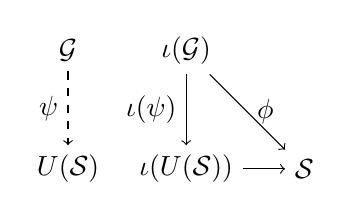
\begin{tikzpicture}
\node (G) at (0,0) {$\mathcal{G}$};
\node (GS) at ([shift={+(0,-1.5)}]G) {$\mathscr{U}(\mathcal{S})$};
\node (iG) at ([shift={+(1.5,0)}]G) {$\iota(\mathcal{G})$};
\node (iGS) at ([shift={+(1.5,-1.5)}]G) {$\iota(\mathscr{U}(\mathcal{S}))$};
\node (S) at ([shift={+(1.5,0)}]iGS) {$\mathcal{S}$};
\draw[->,dashed] (G)--(GS) node[left,midway] {$\psi$};
\draw[->] (iG)--(iGS) node[left,midway] {$\iota(\psi)$};
\draw[->] (iG)--(S) node[right,midway] {$\phi$};
\draw[->] (iGS)--(S) node[below,midway] {$\id$};
\end{tikzpicture}\]
\end{proposition}

\subsection{Quotients}

A somewhat general notion of quotient for discrete semigroupoids is considered in \cite{MR3597709}. We will consider only quotients of inverse semigroupoids which preserve their vertex sets.

\begin{definition}
If $G$ is a graph, an equivalence relation $R$ on $G^{(1)}$ is said to be \emph{graphed} the source and range maps are $R$-invariant (i.e., constant on all $R$-equivalence classes).

A \emph{graph congruence} on an inverse semigroupoid $\mathcal{S}$ is a graphed equivalence relation $R$ on $\mathcal{S}$ such that for all $a,\widetilde{a},b,\widetilde{b}\in \mathcal{S}$, if $(a,\widetilde{a}),(b,\widetilde{b})\in R$ and $(a,b)\in\mathcal{S}^{(2)}$, then $(ab,\widetilde{a}\widetilde{b})\in R$.
\end{definition}

Note that, in the definition above, the product $\widetilde{a}\widetilde{b}$ is defined since $\so(\widetilde{a})=\so(a)=\ra(b)=\ra(\widetilde{b})$, as the source and range maps are constant on $R$-equivalence classes.

Given a graph congruence $R$ on an inverse semigroupoid $\mathcal{S}$, we let $\mathcal{S}/R$ be the \emph{quotient semigroupoid}, which is a graphed semigroupoid constructed in the same manner as quotients of categories (see \cite[Section 2.8]{MR1712872}): The vertex space is $(\mathcal{S}/R)^{(0)}\defeq\mathcal{S}^{(0)}$. The arrow space is the usual quotient set $\mathcal{S}/R$, and we denote the $R$-equivalence class of $a\in\mathcal{S}$ as $[a]$. Since $\so$ and $\ra$ are constant on $R$-equivalence classes, then they factor (uniquely) to maps $\so,\ra\colon\mathcal{S}/R\to\mathcal{S}^{(0)}$, $\so([a])=\so(a)$ and $\ra([a])=\ra(a)$ for all $a\in\mathcal{S}$. The product is defined in the only manner which makes the natural quotient map $\mathcal{S}\to\mathcal{S}/R$ a semigroupoid homomorphism. Namely, given $(x,y)\in (\mathcal{S}/R)^{(2)}$, choose representatives $a\in x$ and $b\in y$. Then $\so(a)=\so(x)=\ra(y)=\ra(b)$, so we may define $xy=[ab]$. Since $R$ is a congruence, this product does not depend on the choice of representatives of $x$ and $y$. Associativity of the product is immediate.

Let us prove that quotients of inverse semigroupoids are also inverse semigroupodis. The following is an analogue of a well-known fact for semigroups, and its proof follows the same steps. See \cite[Theorem 5.1.1]{MR1455373}, for example.

\begin{lemma}[{\cite[Lemma 3.3.1]{MR3597709}}]\label{lem:regularisinverseiffidempotentscommute}
A regular graphed semigroupoid $\mathcal{S}$ is an inverse semigroupoid if and only if elements of $E(\mathcal{S})$ commute, i.e., for all $(e,f)\in (E(\mathcal{S})\times E(\mathcal{S}))\cap \mathcal{S}^{(2)}$, $ef=fe$.
\end{lemma}

The following is a particular case of \cite[Lemma 3.3.3]{MR3597709} and the Lemma above. It may also be proven directly as in the case of inverse semigroups -- see \cite[Proposition 2.1.1(iii)]{MR1724106}.

\begin{proposition}
If $R$ is a graph congruence on an inverse semigroupoid $\mathcal{S}$, then $\mathcal{S}/R$ is an inverse semigroupoid.
\end{proposition}

\subsubsection*{The étale case}

Suppose now that $\mathcal{S}$ is a topological (or étale) inverse semigroupoid, and that $R$ is a graphed congruence on $\mathcal{S}$. We wish to endow $\mathcal{S}/R$ with a natural topology making it a topological (or étale) inverse semigroupoid as well, and for this we use the \emph{quotient topology}. However, in general we do not have control over the topology of $(\mathcal{S}/R)^{(2)}$, and thus we cannot guarantee that the multiplication map of $\mathcal{S}/R$ is continuous with respect to the quotient topology. We will therefore to make further topological assumptions on the congruence $R$ in order to obtain the desired result. Let us briefly recall some facts about quotient topologies.

\begin{itemize}
    \item If $X$ is a topological space, $Y$ is a set, and $\pi\colon X\to Y$ is a function, the \emph{quotient topology} of $Y$ (induced by $\pi$) has as open subsets the subsets $A$ of $Y$ such that $\pi^{-1}(A)$ is open in $X$. In this case, a function $p\colon Y\to Z$, where $Z$ is a topological space, is continuous if and only if $p\circ\pi$ is continuous. In other words, continuous maps from $Y$ are precisely the factors of continuous maps from $X$ through $\pi$.
    \item If $f\colon X\to Y$ is a continuous, open, surjective function between topological spaces, then the topology of $Y$ concides the quotient topology of $f$.
\end{itemize}

Suppose that $R$ is an equivalence relation on a topological space $X$. Given a subset $A\subseteq\mathcal{S}$, we let $R[A]$ denote the \emph{saturation} of $A$, i.e., $R[A]\defeq\left\{x\in X:xRa\text{ for some }a\in A\right\}$. 
We say that $R$ is \emph{open} if the saturation of every open subset of $X$ is open, or equivalently if the quotient map $X\to X/R$ is an open map.

\begin{proposition}\label{prop:equivalecesetalequotient}
Let $\mathcal{S}$ be a topological (resp.\ étale) inverse semigroupoid and $R$ a graphed open congruence on $\mathcal{S}$. Then the quotient topology of $\mathcal{S}/R$ makes it a topological (resp.\ étale) inverse semigroupoid, where we endow $\mathcal{T}^{(0)}=\mathcal{S}^{(0)}$ with its original topology.
\end{proposition}
\begin{proof}
    We first assume only that $\mathcal{S}$ is a topological inverse semigroupoid. Let us denote $\mathcal{T}\defeq\mathcal{S}/R$ and $\pi\colon\mathcal{S}\to\mathcal{T}$ the quotient map.
    
    We have the commutative diagram
    \[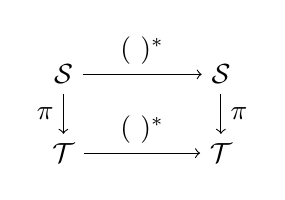
\begin{tikzpicture}
    \node (S1) at (0,0) {$\mathcal{S}$};
    \node (S2) at ([shift={+(2,0)}]S1) {$\mathcal{S}$};
    \node (T1) at ([shift={+(0,-1)}]S1) {$\mathcal{T}$};
    \node (T2) at ([shift={+(2,0)}]T1) {$\mathcal{T}$};
    \draw[->] (S1)--(S2) node[midway,above] {$(\ )^*$};
    \draw[->] (S1)--(T1) node[midway,left] {$\pi$};
    \draw[->] (S2)--(T2) node[midway,right] {$\pi$};
    \draw[->] (T1)--(T2) node[midway,above] {$(\ )^*$};
    \end{tikzpicture}
    \]
    where the horizontal arrows denote the inversion maps. Therefore the inversion map of $\mathcal{T}$ is simply the factor map of $\pi\circ(\ )^*$ through $\pi$, and is therefore continuous. Continuity of the source and range maps may be proven similarly with diagrams.
    
    We will prove that $\mathcal{T}^{(2)}$ has the quotient topology induced by the restriction of $\pi\times\pi$ to $\mathcal{T}^{(2)}$. After that, continuity or the product on $\mathcal{T}$ follows easily, since we have the commutative diagram
    \[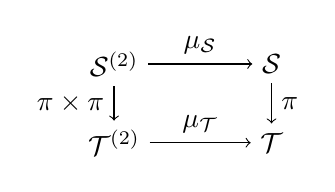
\begin{tikzpicture}
    \node (S2) at (0,0) {$\mathcal{S}^{(2)}$};
    \node (S) at ([shift={+(2,0)}]S2) {$\mathcal{S}$};
    \node (T2) at ([shift={+(0,-1)}]S2) {$\mathcal{T}^{(2)}$};
    \node (T) at ([shift={+(2,0)}]T2) {$\mathcal{T}$};
    \draw[->] (S2)--(S) node[midway,above] {$\mu_{\mathcal{S}}$};
    \draw[->] (S2)--(T2) node[midway,left] {$\pi\times\pi$};
    \draw[->] (S)--(T) node[midway,right] {$\pi$};
    \draw[->] (T2)--(T) node[midway,above] {$\mu_{\mathcal{T}}$};
    \end{tikzpicture}
    \]
    where the horizontal arrows denote the product maps. This means that the product of $\mathcal{T}$ is the factor of a continuous map through $\pi\times\pi$, and is therefore continuous.
    
    Since $\pi$ is surjective, continuous and open, because $R$ is open, then $\pi\times\pi$ is also surjective, continuous and open, and therefore $\mathcal{T}\times\mathcal{T}$ has the quotient topology induced by $\pi\times\pi$.
    
    Moreover, we have $\mathcal{S}^{(2)}=(\pi\times\pi)^{-1}\left(\mathcal{T}^{(2)}\right)$ and so for every $A\subseteq \mathcal{S}\times\mathcal{S}$ we have $(\pi\times\pi)(A\cap\mathcal{S}^{(2)})=(\pi\times\pi)(A)\cap\mathcal{T}^{(2)}$. In particular the restriction $(\pi\times\pi)|_{\mathcal{S}^{(2)}}\colon\mathcal{S}^{(2)}\to\mathcal{T}^{(2)}$ is also continuous, surjective, and open, and therefore $\mathcal{T}^{(2)}$ has its quotient topology, and continuity of the product map follows.
    
    Now assume that $\mathcal{S}$ is étale. If $A$ is an open bisection of $\mathcal{S}$, then $\pi(A)$ is an open bisection of $\mathcal{T}$, because $\so_{\mathcal{T}}\circ\pi=\so_{\mathcal{S}}$ and $\ra_{\mathcal{T}}\circ\pi=\ra_{\mathcal{S}}$ are injective on $A$. Moreover, the source map of $\mathcal{T}$ is open: if $C\subseteq\mathcal{T}$ is open, then $\so_{\mathcal{T}}(C)=\so_{\mathcal{S}}(\pi^{-1}(C))$ is open in $\mathcal{T}^{(0)}=\mathcal{S}^{(0)}$. Therefore $\so_{\mathcal{T}}$ is continuous, open, and locally injective, hence a local homeomorphism.\qedhere
\end{proof}

Therefore, under the hypotheses of Proposition \ref{prop:equivalecesetalequotient}, $\pi\colon\mathcal{S}\to\mathcal{S}/R$ is a continuous homomorphism of topological inverse semigroupoid satisfying the usual universal property: If $\phi\colon\mathcal{S}\to\Lambda$ is any continuous (resp.\ open) homomorphism from $\mathcal{S}$ to a topological semigroupoid $\Lambda$ such that $R\subseteq\ker\phi$, then there exists a unique continuous (resp.\ open) semigroupoid homomorphism $\psi\colon\mathcal{S}/R\to\Lambda$ such that $\phi=\psi\circ\pi$.

\begin{denv*}{Remark}
A similar construction as in \cite{MR0412333} shows, by set-theoretic considerations, that the category of topological inverse semigroupoids admits arbitrary quotients in the following sense: If $\mathcal{S}$ is any topological inverse semigroupoid and $R$ is any congruence on $\mathcal{S}$, then there exists a topological inverse semigroupoid $\mathcal{S}/R$ and a continuous homomorphism $\pi_R\colon\mathcal{S}\to\mathcal{S}/R$ such that $\pi_R(a)=\pi_R(b)$ whenever $(a,b)\in R$, and for any other inverse semigroupoid $\mathcal{T}$ and any continuous homomorphism $\phi\colon\mathcal{S}\to\mathcal{T}$ such that $\phi(a)=\phi(b)$ whenever $(a,b)\in R$, then there exists a unique continuous groupoid homomorphism $\psi\colon\mathcal{S}/R\to\mathcal{T}$ such that $\psi\circ\pi_R=\phi$.

The main idea in the construction of $\mathcal{S}/R$ as above is to show that there is a set $\mathscr{Q}$ of all possible topological semigroupoid quotients of $\mathcal{S}$ which identify $R$-equivalent elements of $\mathcal{S}$. More precisely, $\mathscr{Q}$ is a set of topological inverse semigroupoids $Q$ endowed with continuou maps $\pi_Q\colon\mathcal{S}\to Q$ such that $\pi_Q(a)=\pi_Q(b)$ whenever $(a,b)\in R$, and which satisfies the following property: If $\phi\colon\mathcal{S}\to\mathcal{T}$ is any topological semigroupoid homomorphism such that $\phi(a)=\phi(b)$ whenever $(a,b)\in R$ and $\phi(\mathcal{S})$ generates $\mathcal{T}$ (as an inverse semigroupoid), then $(\mathcal{T},\phi)$ may be represented (faithfully) as $(Q,\pi_Q)$ for some $Q\in\mathscr{Q}$. We then take $(\mathcal{S}/R)'=\prod_{Q\in\mathscr{Q}}Q$, $\pi=\prod_{Q\in\mathscr{Q}}\pi_Q$, and $\mathcal{S}/R$ the sub-inverse semigroupoid of $(\mathcal{S}/R)'$ generated by $\pi(S)$.

However, the topology of $\mathcal{S}/R$ is not manageable in abstract terms, and a priori the inverse semigroupoid $\mathcal{S}/R$ might be trivial even if $R\neq\mathcal{S}\times\mathcal{S}$.
\end{denv*}

\subsection{Semigroupoids of germs and the initial groupoid}\label{subsec:groupoidofgerms}

\begin{definition}
A poset $(P,\preceq)$ is \emph{conditionally downwards directed} for all $p\leq P$, the downset $p^{\downarrow,\preceq}=\left\{x\in P:x\preceq p\right\}$ is downwards directed. Explicitly, this means that whenever $x,y\preceq p$ in $P$, there exists $z\in P$ with $z\preceq x,y$.
\end{definition}

As an example, every inverse semigroupoid with its canonical order is conditionally downwards directed.

The \emph{germ relation} $\sim_{\preceq}$ on a poset $(P,\preceq)$ is defined as
\[a\sim_{\preceq} b\iff\text{there exists }z\in P\text{ such that } z\leq a\text{ and }z\leq b.\]

\begin{lemma}
$\sim_\preceq$ is always reflexive and symmetric, and it is transitive (and thus an equivalence relation) if and only if $(P,\preceq)$ is conditionally downwards directed.
\end{lemma}
\begin{proof}
    Only the last statement warrants a proof. If $(P,\preceq)$ is conditionally downwards directed, then suppose $a\sim_{\preceq} b$ and $b\sim_{\preceq} c$. Let $x$ and $y$ with $x\preceq a,b$ and $y\preceq b,c$. As both $x$ and $y$ are bounded above by $b$, we may take $z\preceq x,y$. Then $z\preceq x\preceq a$ and $z\preceq y\preceq c$, so $a\sim_\preceq c$. Hence $\sim_\preceq$ is transitive.
    
    Conversely, if $\sim_\preceq$ is transitive, suppose $x,y\preceq p$ in $P$. Then $x\sim_\preceq p$ and $p\sim_\preceq y$, so $x\sim_\preceq y$, which means that there exists $z\preceq x,y$, as desired.\qedhere
\end{proof}

The following example will be used in our duality result, and yields a large class 

\begin{definition}\label{def:compatibleorder}
    A preorder $\preceq$ on a semigroupoid $\mathcal{S}$ is \emph{compatible} (with $\mathcal{S}$) if
    \begin{enumerate}[label=(\roman*)]
        \item\label{def:compatibleorder1} $a\preceq b$ implies $a\leq b$;
        \item\label{def:compatibleorder2} $a\preceq b$ implies $ax\preceq bx$ and $ya\preceq yb$ whenever $(a,x),(y,a)\in\mathcal{S}^{(2)}$.
    \end{enumerate}
    (note that $bx$ and $yb$ in \ref{def:compatibleorder2} are defined because, by \ref{def:compatibleorder1}, $a\leq b$, so $\so(a)=\so(b)$ and $\ra(a)=\ra(b)).$
\end{definition}

Any compatible preorder $\preceq$ on a semigroupoid $\mathcal{S}$ is preserved by inverses: If $a\preceq b$, then $a\leq b$, so
\[a^*=b^*ab^*\preceq b^*bb^*=b^*\]

\begin{example}\label{ex:setorderofbisections}.
    Let $\mathcal{S}$ be an étale inverse semigroupoid and let $\mathbf{B}(\mathcal{S})$ be its semigroup of open bisections. Then set inclusion $\subseteq$ is a compatible preorder compatible with $\mathbf{B}(\mathcal{S})$. Set inclusion coincides with the canonical order of $\mathbf{B}(\mathcal{S})$ if and only if $\mathcal{S}$ is a groupoid.
    
    Indeed, suppose that $\mathcal{S}$ is not a groupoid. Then the canonical order of $\mathcal{S}$ is not equality, i.e., there are $a\neq b$ in $\mathcal{S}$ with $a\leq b$. Take any two open bisections $A_0,B_0\in\mathbf{B}(\mathcal{S})$ containing $a$ and $b$, respectively. Then $A\defeq A_0\cap B_0^{\uparrow,\leq}$ and $B\defeq B_0\cap A^{\downarrow,\leq}$ are also open bisections of $\mathcal{S}$ containing $a$ and $b$, respectively (see Corollary \ref{cor:propertiesopeninversesemigroupoid}). However, $B\leq A$ in the canonical order of $\mathbf{B}(\mathcal{S})$, but $B$ is not contained in $A$.
    
    The verification of the other direction -- that if $\mathcal{G}$ is an étale groupoid then the canonical order of $\mathbf{B}(\mathcal{G})$ is set inclusion -- is straightforward.
\end{example}

\begin{lemma}\label{lem:relation.of.germs.is.a.graphed.congruence}
If $\preceq$ is a compatible preorder on an inverse semigroupoid $\mathcal{S}$ then it is conditionally downwards directed, and $\sim_{\preceq}$ is a graphed congruence.
\end{lemma}
\begin{proof}
    To prove that $\preceq$ is conditionally downwards directed, suppose $x,y\preceq a$. Then $x,y\leq a$ as well. The product $z\defeq xy^*y$ is thus defined, and
    \[z=xy^*y\preceq ay^*y=y,\qquad\text{and}\qquad z=xy^*y\preceq xa^*a=x.\]
    (In fact, note that any $\preceq$-lower bound $w$ of $\left\{x,y\right\}$ satisfies $w=ww^*w\preceq xy^*y=z$, so $z=\inf_{\preceq}\left\{x,y\right\}$.)
    
    Property \ref{def:compatibleorder}\ref{def:compatibleorder1} implies that the source and range maps are $\sim_{\preceq}$-invariant, so $\sim_{\preceq}$ is graphed. If $a_i\sim_{\preceq} b_i$ ($i=1,2$) and $(a_1,a_2)\in\mathcal{S}^2$, we choose $c_i\preceq a_i,b_i$, so applications of \ref{def:compatibleorder}\ref{def:compatibleorder1} imply $c_1c_2\preceq a_1a_2$ and $c_1c_2\preceq b_1b_2$, thus $a_1a_2\sim_{\preceq} b_1b_2$, which proves that $\sim_{\preceq}$ is a congruence.\qedhere
\end{proof}

\begin{denv*}{Remark}
The germ relation associated to a compatible order does not determine the order completely. For example, let $L_3=\left\{0,1,2\right\}$ be the lattice with $0<1<2$. Set $x\preceq y$ if and only if $x=y$ or $x=a$. Then $\preceq$ is a compatible order on $L_3$, different from the canonical order $\leq$ but with the same germ relation (namely, all elements of $L_3$ are equivalent).
\end{denv*}

Therefore, given an inverse semigroupoid $\mathcal{S}$ and a compatible order $\preceq$, we may construct the quotient inverse semigroupoid $\mathcal{S}/\!\!\sim_{\preceq}$. If $\mathcal{S}$ is étale, we wish to apply Proposition \ref{prop:equivalecesetalequotient} to make $\mathcal{S}/\!\!\sim_{\preceq}$ étale as well.

\begin{definition}
A \emph{topologically compatible} order $\preceq$ on a topological inverse semigroupoid $\mathcal{S}$ is a compatible order $\preceq$ such that upper and lower closures of open sets are also open, i.e., if $A\subseteq\mathcal{S}$ is open, then
\[A^{\uparrow,\preceq}=\left\{z\in\mathcal{S}:a\preceq z\text{ for some }a\in A\right\}\quad\text{and}\quad A^{\downarrow,\preceq}=\left\{z\in\mathcal{S}:z\preceq a\text{ for some }a\in A\right\}\]
are open in $\mathcal{A}$.
\end{definition}

\begin{example}
Let $X=[0,1]$ as a unit topological groupoid and its usual topology. Consider the discrete lattice $L_2=\left\{0,1\right\}$ with $0<1$ and the topological semigroupoid $\mathcal{S}\defeq L_2\times X$. Then $\mathcal{S}$ is an étale inverse semigroupoid. The order
\[x\preceq y\iff x=y\text{ or }x=(0,1)\text{ and }y=(1,1)\]
is compatible but not topologically compatible with $\mathcal{S}$. Moreover, it is not hard to verify that the quotient $\mathcal{S}/\!\!\sim_{\preceq}$ is a topological, non-étale, inverse semigroupoid when endowed with the quotient topology.
\end{example}

At this moment, we do not have an example of a compatible order $\preceq$ on a topological inverse semigroupoid $\mathcal{S}$ such that the product map on $\mathcal{S}/\!\!\sim_{\preceq}$ is not continuous with respect to the quotient topology.

Given a topologically compatible order $\preceq$ on a topological inverse semigroupoid $\mathcal{S}$, the $\sim_{\preceq}$-saturation of an open subset $A\subseteq\mathcal{S}$ is
\[\sim_{\preceq}[A]=(A^{\downarrow,\preceq})^{\uparrow,\preceq}.\]
which is open. Therefore $\sim_{\preceq}$ is open, and as a particular case of Proposition \ref{prop:equivalecesetalequotient}, we obtain the following result.

\begin{proposition}
Suppose that $\preceq$ is a topologically compatible order on a topological (resp.\ étale) inverse semigroupoid $\mathcal{S}$. Then the quotient topology on $\mathcal{T}=\mathcal{S}/\!\!\sim_{\preceq}$ makes it a topological (resp.\ étale) inverse semigroupoid. (We endow $\mathcal{S}^{(0)}=\mathcal{T}^{(0)}$ with its original topology.)
\end{proposition}

Given an étale inverse semigroupoid $\mathcal{S}$, the canonical order $\leq$ of $\mathcal{S}$ is topologically compatible, by Corollary \ref{cor:propertiesopeninversesemigroupoid}\ref{cor:propertiesopeninversesemigroupoid2}, and thus we may apply the result above.

\begin{definition}
    The \emph{initial groupoid} of an étale inverse semigroupoid is the topological (semi)groupoid $\IG(\mathcal{S})=\mathcal{S}/\!\!\sim_{\leq}$.
\end{definition}

To check that $\IG(\mathcal{S})$ is indeed a groupoid, we may simply verify that its canonical order is trivial. Denote by $\pi_{\mathcal{S}}\colon\mathcal{S}\to\IG(\mathcal{S})$ the (usual) quotient map. If $\pi_{\mathcal{S}}(a)\leq\pi_{\mathcal{S}}(b)$, then $\pi_{\mathcal{S}}(a)=\pi_{\mathcal{S}}(ba^*a)$. Since $ba^*a\leq b$ then $ba^*a$ and $b$ are $\sim_{\leq}$ related, hence $\pi_{\mathcal{S}}(b)=\pi_{\mathcal{S}}(ba^*a)=\pi_{\mathcal{S}}(a)$.

Moreover, $\IG(\mathcal{S})$ satisfies a universal property for semigroupoid homomorphisms from $\mathcal{S}$ to topological groupoids (and hence its name): Let $\pi_{\mathcal{S}}\colon\mathcal{S}\to\IG(\mathcal{S}$ be the canonical quotient map. Suppose that $\phi\colon\mathcal{S}\to\mathcal{G}$ is a continuous semigroupoid homomorphism, where $\mathcal{G}$ is a topological groupoid. As $\phi$ preserves the orders and the order of $\mathcal{G}$ is trivial, then $\phi$ is $\sim_{\leq}$-invariant, and thus $\phi$ factors through $\pi_\mathcal{S}$ to a continuous groupoid homomorphism $\psi\colon \IG(\mathcal{S})\to\mathcal{G}$, i.e., $\phi=\psi\circ\pi_{\mathcal{S}}$.

In particular, if $\mathcal{T}$ is another étale inverse semigroupoid and $\phi\colon\mathcal{S}\to\mathcal{T}$ is a continuous semigroupoid homomorphism, then the composition $\pi_T\circ\phi\colon\mathcal{S}\to\IG(\mathcal{T})$ factors uniquely through $\IG(\mathcal{S})$, so we obtain a continuous groupoid homomorphism $\IG(\phi)\colon\IG(\mathcal{S})\to\IG(\mathcal{T})$. Therefore we have a functor $\IG\colon\cat{EtIS}\to\cat{EtGr}$, and the previous paragraph proves that it is initial with respect to the inclusion of categories $\iota\colon\cat{EtGr}\hookrightarrow\cat{EtIS}$.

\begin{proposition}
Let $\mathcal{S}$ be an étale inverse semigroupoid. Then for every étale groupoid $\mathcal{G}$, every continuous semigroupoid morphism $\phi\colon \mathcal{S}\to\mathcal{G}$ factors through a continuous groupoid homomorphism $\IG(\mathcal{S})\to\mathcal{G}$. In other words, there exists a unique continuous groupoid homomorphism $\psi\colon\IG(\mathcal{S})\to\mathcal{G}$ such that the following diagram commutes:
\[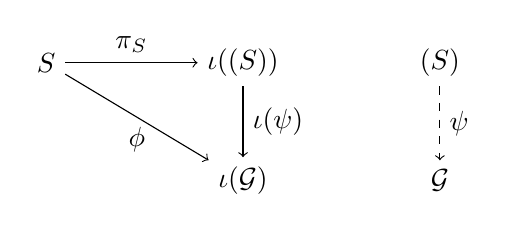
\begin{tikzpicture}
\node (S) at (0,0) {$S$};
\node (igS) at ([shift={+(2.5,0)}]S) {$\iota(\IG(S))$};
\node (iG) at ([shift={+(0,-1.5)}]igS) {$\iota(\mathcal{G})$};
\node (gS) at ([shift={+(2.5,0)}]igS) {$\IG(S)$};
\node (G) at ([shift={+(0,-1.5)}]gS) {$\mathcal{G}$};
\draw[->,dashed] (gS)--(G) node[right,midway] {$\psi$};
\draw[->] (igS)--(iG) node[right,midway] {$\iota(\psi)$};
\draw[->] (S)--(igS) node[above,midway] {$\pi_S$};
\draw[->] (S)--(iG) node[below,midway] {$\phi$};
\end{tikzpicture}\]
\end{proposition}

If $\mathcal{G}$ is a groupoid, then its order is trivial and the associated germ relation is the identity, hence the restriction of $\IG$ to $\cat{EtGr}$ is naturally isomorphic to the identity functor. In this manner, $\IG$ may also be regarded as a retraction from $\cat{EtIS}$ onto its full subcategory $\cat{EtGr}$.

\begin{example}
If $S$ is a discrete inverse semigroup, then $\IG(S)$ is called the \emph{maximal group homomorphic image} of $S$. See \cite[Proposition 2.1.2]{MR1724106}.
\end{example}

\begin{example}
If $\theta\colon S\curvearrowright X$ is a continuous $\land$-preaction of an inverse semigroup $S$ on a topological space $X$, then we have seen in Example \ref{ex:semidirectproductofactionisetale} the semidirect product $S\ltimes X$ is an étale inverse semigroupoid. The groupoid $\IG(S\ltimes X)$ is the \emph{groupoid of germs} of $\theta$, as considered in \cite{arxiv1804.00396}.
\end{example}

\subsubsection*{Quotients of semidirect products}

Let $(\pi,\theta)\colon\mathcal{S}\curvearrowright\mathcal{T}$ be an open, continuous $\land$-preaction, where $\mathcal{S}$ and $\mathcal{T}$ are topological inverse semigroupoids. We will now analyse how the operations of ``taking quotients'' and ``taking semidirect products'' behave with respect to each other. Abusing language, we might simply say that ``quotients and semidirect products commute''.

Suppose that $R_1$ and $R_2$ are graphed congruences on $\mathcal{S}$ and $\mathcal{T}$, respectively. We denote equivalence classes, either in $\mathcal{S}$ or $\mathcal{T}$, simply by brackets, if $a\in\mathcal{S}$ then $[a]$ denotes its $R_1$-equivalence class, and similarly in $\mathcal{T}$.

On one direction, consider the equivalence relation $R_1\times R_2$ on $\mathcal{S}\ltimes\mathcal{T}$ -- namely $(s_1,t_1)$ is $(R_1\times R_2)$-equivalent to $(s_2,t_2)$ if and only if $s_1$ is $R_1$-equivalent to $s_2$ and $t_1$ is $R_2$-equivalent to $t_2$. We wish that $R_1\times R_2$ is a congruence on $\mathcal{S}\ltimes\mathcal{T}$, and for this we need to impose conditions on the congruences $R_1$ and $R_2$.

The $(R_1\times R_2)$-class of $(a,x)\in\mathcal{S}\ltimes\mathcal{T}$ is denoted $[a,x]$.

\begin{definition}
    A graphed congruence $R$ on an inverse semigroupoid $R$ is \emph{idempotent pure} if $(a,e)\in R$ and $e\in E(\mathcal{S})$ implies $a\in\mathcal{E(\mathcal{S})}$ (i.e., the saturation of $E(\mathcal{S})$ is $E(\mathcal{S})$).
\end{definition}

The following equivalences are well-known in the case of inverse semigroups, and the proofs are easy enough, so we omit them.

\begin{proposition}\label{prop:equivalencesidempotentpure}
The following are equivalent:
\begin{enumerate}[label=(\roman*)]
    \item\label{prop:equivalencesidempotentpure1} $R$ is idempotent pure;
    \item\label{prop:equivalencesidempotentpure2} The canonical quotient map $\pi\colon\mathcal{S}\to\mathcal{S}/R$ is idempotent pure, in the sense that $\pi^{-1}(E(\mathcal{S}/R))=E(\mathcal{S})$.
    \item\label{prop:equivalencesidempotentpure3} If $(a,b)\in R$, then $a^*b\in E(\mathcal{S})$ (and also $ab^*\in E(\mathcal{S})$);
\end{enumerate}
\end{proposition}

We therefore make two standing hypotheses on the congruence $R_1$ and $R_2$, and the action $(\pi,\theta)$.

\begin{enumerate}[label=(H\arabic*)]
\item\label{hyp:onrelationsforsemidirectproduct1} $R_1$ is idempotent pure;
\item\label{hyp:onrelationsforsemidirectproduct2} $\theta$ is an $R_2$-morphism: For all $a\in\mathcal{S}$ and $x,y\in\dom(\theta_a)$, if $(x,y)\in R_2$ then $(\theta_a(x),\theta_a(y))\in R_2$.
\end{enumerate}

\begin{lemma}\label{lem:hypmakeformulasgood}
Under hypotheses \ref{hyp:onrelationsforsemidirectproduct1} and \ref{hyp:onrelationsforsemidirectproduct2}, $(R_1\times R_2)$ is a graphed congruence on $\mathcal{S}\ltimes\mathcal{T}$. Moreover, if $[a,x]=[b,y]$ then $[\theta_a(x)]=[\theta_b(y)]$.
\end{lemma}
\begin{proof}
    We start with the last statement. Suppose $[a,x]=[b,y]$. Then
    $[x]=[y]=[xy^*y]$, and $xy^*y$ belongs to both $\dom(\theta_a)$ and $\dom(\theta_b)$. As $R_1$ is idempotent pure, $\theta_a$ and $\theta_b$ are compatible, and thus coincide on the intersection of their domains. Since $\theta$ is an $R_2$-morphism then
    \[[\theta_a(x)]=[\theta_a(xy^*y)]=[\theta_b(xy^*y)]=[\theta_b(y)],\]
    as desired.
    
    We can now prove that the source and range maps of $\mathcal{S}\ltimes\mathcal{T}$ are $R_1\times R_2$-invariant. Assuming $[a,x]=[b,y]$, we have $[\theta_a(x)]=[\theta_b(y)]$ by the previous paragraph. As $R_2$ is graphed,
    \[\ra(a,x)=\ra(\theta_a(x))=\ra(\theta_b(y))=\ra(b,y).\]
    and $\so(a,x)=\so(x)=\so(y)=\so(b,y)$.
    
    It remains only to prove that if $[a,x]=[b,y]$, $[c,z]=[d,w]$, and the product $(a,x)(c,z)$ is defined, then $[(a,x)(c,z)]=[(b,y)(d,w)]$. More specifically, we need to prove that
    \[[ac,\theta_c^{-1}(x\theta_c(z))]=[bd,\theta_d^{-1}(y\theta_d(w))]\]
    Again using the last part of the lemma, we have $[\theta_c(z)]=[\theta_d(w)]$, so $[x\theta_c(z)]=[y\theta_d(w)]$ because $R_2$ is a congruence. Applying the last part one more time yields
    \[[\theta_c^{-1}(x\theta_c(z))]=[\theta_d^{-1}(y\theta_d(w))]\]
    and also $[ac,bd]$ because $R_1$ is a congruence.\qedhere
\end{proof}

The lemma above allows us to construct the quotient of the semidirect product, $(\mathcal{S}\ltimes\mathcal{T})/R_1\times R_2$. We now do the opposite, namely we construct a semidirect product of the quotients, $(\mathcal{S}/R_1)\ltimes(\mathcal{T}/R_2)$. First we need to describe the $\land$-preaction of $\mathcal{S}/R_1$ on $\mathcal{T}/R_2$.

The anchor map $\pi\colon\mathcal{T}\to\mathcal{S}^{(0)}$ is a homomorphism, so if $\ra(x)=\ra(y)$, then $x^*y$ is defined, so $\pi(x)=\pi(x^*)=\pi(y)$. Since $R_2$ is graphed then $\pi$ factors unique to a homomorphism, $\mathcal{T}/R_2\to\mathcal{S}^{(0)}$, which we also denote $\pi$.

We now define the action of $\mathcal{S}/R_1$ on $\mathcal{T}/R_2$, which we denote by $\Theta$. Given an $R_1$-class $\alpha\in\mathcal{S}/R_1$, consider the subsets of $\mathcal{T}/R_2$
\[D_\alpha\defeq\left\{[x]:x\in\dom(\theta_b)\text{ for some }b\in\mathcal{S}\text{ with }(b,\alpha)\in R_1\right\}.\]
and
\[R_\alpha\defeq\left\{[x]:x\in\ran(\theta_b)\text{ for some }b\in\mathcal{S}\text{ with }(b,\alpha)\in R_1\right\}.\]
Note that $R_\alpha=D_{\alpha^*}$, and that $D_\alpha$ is a subset of $\pi^{-1}(\so(\alpha))$.

By Lemma \ref{lem:hypmakeformulasgood}, we may define a map $\Theta_{\alpha}\colon D_\alpha\to R_\alpha$ by
\[\Theta_\alpha([x])=[\theta_a(x)],\qquad\text{ whenever }a\in\alpha\text{ and }x\in\dom(\theta_a).\]
We have already seen that if $a,b\in\alpha$ then $\theta_a$ and $\theta_b$ coincide on their common domain, and from this it follows that $\Theta_\alpha$ is a bijection from $D_\alpha$ to $R_\alpha$. We will prove that it is a $\land$-preaction, in the sense of Definition \ref{def:partialactiononsemigroupoid}. For this, let us make a small detour to the theory of \emph{$\lor$-prehomomorphisms}, which are dual to $\land$-prehomomorphisms.

\begin{definition}
A \emph{$\lor$-prehomomorphism} between inverse semigroupoids is a map $\theta\colon\mathcal{S}\to\mathcal{T}$ which satisfies $(\theta\times\theta)(\mathcal{S}^{(2)})\subseteq\mathcal{T}^{(2)}$ and $\theta(ab)\leq\theta(a)\theta(b)$ whenever $(a,b)\in\mathcal{S}^{(2)}$.
\end{definition}

\begin{proposition}\label{prop:invertiblelorprehomarehom}
If $\theta\colon\mathcal{S}\to\mathcal{T}$ is a $\land$-prehomomorphism, then $\theta$ preserves idempotents, the canonical order, and inverses.

If $\theta$ is invertible and $\theta^{-1}$ is also a $\lor$-prehomomorphism, then $\theta$ is an isomorphism.
\end{proposition}
\begin{proof}
    The statements in the first paragraph may be proven just as in the case of inverse semigroups; see \cite[Proposition 3.1.5]{MR1694900}. Let us prove the last statement. Suppose $\theta$ is invertible and $\theta^{-1}$ is also a $\lor$-prehomomorphism.
    
    Given $(a,b)\in\mathcal{S}^{(2)}$, we have
    \[\theta(ab)\leq\theta(a)\theta(b).\]
    Since $\theta^{-1}$ is a $\lor$-prehomomorphism, and in particular it preserves the order,
    \[ab\leq\theta^{-1}(\theta(a)\theta(b))\leq\theta^{-1}(\theta(a))\theta^{-1}(\theta(b))=ab\]
    so $ab=\theta^{-1}(\theta(a)\theta(b))$, or equivalently, $\theta(ab)=\theta(a)\theta(b)$.\qedhere
\end{proof}

\begin{proposition}
If $(\pi,\theta)$ is a $\land$-preaction then $(\pi,\Theta)$ is a $\land$-preaction.
\end{proposition}
\begin{proof}
    We simply need to verify that if $(\pi,\theta)$ satisfies any of properties \ref{def:dualprehomomorphismandpartialhomomorphism}\ref{def:dualprehomomorphismandpartialhomomorphism1}, \ref{def:dualprehomomorphismandpartialhomomorphism2} or \ref{def:dualprehomomorphismandpartialhomomorphism3}, then $(\pi,\Theta)$ satisfies the same property.
    
    The work for \ref{def:dualprehomomorphismandpartialhomomorphism}\ref{def:dualprehomomorphismandpartialhomomorphism1} is straightforward, i.e., if $\theta_a^{-1}=\theta_{a^*}$ for all $a\in\mathcal{S}$, then $\Theta_\alpha^{-1}=\Theta_{\alpha^*}$.
    
    Assume then that $(\pi,\theta)$ satisfies \ref{def:dualprehomomorphismandpartialhomomorphism}\ref{def:dualprehomomorphismandpartialhomomorphism2}: For all $(a,b)\in\mathcal{S}^{(2)}$, $\theta_a\circ\theta_b\leq\theta_{ab}$.
    
    Suppose $(\alpha,\beta)\in(\mathcal{S}/R_1)^{(2)}$ and $\gamma\in\dom(\Theta_\alpha\circ\Theta_\beta)$. Then we can find $b\in\beta$ and $x\in\gamma\cap\dom(\theta_b)$ such that $\Theta_\beta(\gamma)=[\theta_b(x)]$, and this belongs to $\dom(\Theta_\alpha)$. Then, find $a\in\alpha$ and $y\in\dom(\theta_a)$ such that $[\theta_b(x)]=[y]$ and $\Theta_\alpha(\Theta_\beta(\gamma))=[\theta_a(y)]$.
    
    We have $[y]=[\theta_b(x)]=[\theta_b(x)y^*y]$, and the element $\theta_b(x)y^*y$ belongs to both $\ran(\theta_b)$ and $\dom(\theta_a)$. Then we can consider $z\in\dom(\theta_b)$ (namely, $z=\theta_{b^*}(\theta_b(x)y^*y)$) such that $\theta_b(x)y^*y=\theta_b(z)$. Moreover, as $[\theta_b(x)]=[\theta_b(z)]$ then $[x]=[z]$, because $\theta$ is an $R_2$-morphism. Then $z\in\dom(\theta_a\circ\theta_b)$, so $\gamma=[z]\in\dom(\Theta_\alpha\circ\Theta_\beta)$, and
    \[\Theta_\alpha(\Theta_\beta(\gamma))=\Theta_\alpha([\theta_b(z)])=[\theta_a(\theta_b(z))]=[\theta_{ab}(z)]=\Theta_{\alpha\beta}(\gamma).\]
    This proves that $\Theta_\alpha\circ\Theta_\beta\leq\Theta_{\alpha\beta}$, as we wanted.
    
    It remain only to prove that each map $\Theta_\alpha$ is an isomorphism between ideals of $\mathcal{T}/R_2$. It should be clear that $D_\alpha$ is an ideal for each $\alpha\in\mathcal{S}/R_1$. Moreover, recall that as $R_2$ is graphed, then a product $[x][y]$ is defined in $\mathcal{T}/R_2$ if and only if $xy$ is defined in $\mathcal{T}$, in which case $[x][y]=[xy]$.
    
    Let $\alpha\in\mathcal{S}/R_1$. First we prove that $\Theta_\alpha$ preserves idempotents. Indeed, if $\gamma\in\dom(\Theta_\alpha)$ is idempotent, take $a\in\alpha$ and $x\in\gamma\cap\dom(\theta_a)$. As $[x]=\gamma=\gamma^*\gamma=[x^*x]$, we may assume that $x\in E(\mathcal{S})$, so $\theta_a(x)\in\mathcal{E}(\mathcal{T})$, because $\theta_a$ is an isomorphism, and thus $\Theta_\alpha(\gamma)=[\theta_a(x)]\in E(\mathcal{T}/R_2)$.
    
    We may now prove that $\Theta_{\alpha}$ is a $\lor$-prehomomorphism. Suppose that $\gamma,\delta\in\dom(\Theta_\alpha)$. Then are $a,b\in\alpha$ and $x\in\gamma\cap\dom(\theta_a)$ and $y\in\delta\cap\dom(\theta_b)$. If $\gamma\delta$ is defined and it also belongs to $\dom(\Theta_\alpha)$, so there is $c\in\alpha$ and $z\in(\gamma\delta)\cap\dom(\theta_c)$. We then apply Lemma \ref{lem:hypmakeformulasgood} several times, which allows us to compute
    \begin{align*}
        \Theta_\alpha(\gamma\delta)&=[\theta_c(z)]=[\theta_a(xy)]=[\theta_a(x)][\theta_a(x^*xy)]=\Theta_\alpha(\gamma)[\theta_b(x^*xy)]=\Theta_\alpha(\gamma)[\theta_b(x^*xyy^*)][\theta_b(y)]\\
        &=\Theta_\alpha(\gamma)\Theta_\alpha([x^*xyy^*])\Theta_\alpha(\delta).
    \end{align*}
    Since $\Theta_\alpha$ preserves idempotents, then $\Theta_\alpha(\gamma\delta)\leq\Theta_\alpha(\gamma)\Theta_\alpha(\delta)$, so $\Theta_\alpha$ is a $\lor$-prehomomorphism. The same holds for $\Theta_{\alpha^*}=\Theta_\alpha^{-1}$, so by Proposition \ref{prop:invertiblelorprehomarehom}, $\Theta_\alpha$ is an isomorphism.\qedhere.
\end{proof}

\begin{denv*}{Remark}
    The analogous result to the proposition above for partial actions is not true. The following example was considered in \cite[Example 4.5]{Mikola2017}. Let $E=\left\{0,a,b\right\}$ be the semilattice with $x\leq y$ if and only if $x=0$ or $x=y$, acting on the lattice $L_2=\left\{0,1\right\}$, where $0<1$, as follows: $\theta_0$ and $\theta_a$ are the identity of $\left\{0\right\}$ and $\theta_b=\id_{L_2}$. Then, in fact, $\theta$ is a global action.
    
    We let $R_1$ be the congruence which identifies $0$ and $b$ in $E$, and $R_2$ the identity of $L_2$. Again denoting by $\Theta$ the $\land$-preaction of $E/R_1$ on $L_2/R_2\cong T$, we have $[0]\leq[a]$, but $\Theta_{[0]}=\theta_b$, $\Theta_{[a]}=\theta_a$, and $\theta_a<\theta_b$.
\end{denv*}

We will now consider the topological setting. The two standing hypotheses \ref{hyp:onrelationsforsemidirectproduct1} and \ref{hyp:onrelationsforsemidirectproduct2} are still maintained.

\begin{lemma}\label{lem:topologicalpropertiesofacctionpasstoquotients}
Suppose that $\mathcal{S}$ is étale, $\mathcal{T}$ is topological, $(\pi,\theta)$ is a continuous open $\land$-preaction, and $R_1$ and $R_2$ are open. Let $\pi_1\colon\mathcal{S}\to\mathcal{S}/R_1$, $\pi_2\colon\mathcal{T}\to\mathcal{T}/R_2$ be the canonical quotient maps. Then
\begin{enumerate}[label=(\alph*)]
    \item\label{lem:topologicalpropertiesofacctionpasstoquotients1} $\pi_1\times\pi_2\colon\mathcal{S}\ltimes\mathcal{S}\to(\mathcal{S}/R_1)\ltimes(\mathcal{T}/R_2)$ is surjective, continuous and open. In particular, $(\mathcal{S}/R_1)\ltimes(\mathcal{T}/R_2)$ carries the quotient topology of $\pi_1\times\pi_2$.
    \item\label{lem:topologicalpropertiesofacctionpasstoquotients2} $R_1\times R_2$ is open.
    \item\label{lem:topologicalpropertiesofacctionpasstoquotients3} $(\pi,\Theta)$ is open and continuous.
\end{enumerate}
\end{lemma}
\begin{proof}
    Consider the map $p\colon\mathcal{S}\ltimes\mathcal{T}\to\mathcal{T}$, $p(a,x)=x$, which we know to be a from Proposition \ref{prop:preactionisopeniffprojectionisopen}.
    \begin{enumerate}[label=(\alph*)]
    \item Surjectivity and continuity of $\pi_1\times\pi_2$ should be clear, so we prove that it is open. A basic open set of $\mathcal{S}\ltimes\mathcal{T}$ has the form $A\ast U$, where $A$ is an open bisection of $\mathcal{S}$ and $U$ is open in $\mathcal{T}$. Let us prove that
    \[(\pi_1\times\pi_2)(A\ast U)=\pi_1(A)\ast\pi_2(p(A\ast U)).\ntag\label{eq:proofofisomorphismofquotientandsemidirectproduct}\]
    Indeed, the inclusion ``$\subseteq$'' is immediate. Conversely, an element of the right-hand side may be writtens in the form $([a],[x])$, where $x\in\dom(\theta_b)$ for some $b\in A$, and also in the form $([c],[z])$ where $z\in\dom(\theta_c)$. As $R_2$ is graphed then $\ra(x)=\ra(z)$, so $\pi(x)=\pi(z)$. As $R_1$ is also graphed, then
    \[\so(a)=\so(c)=\pi(z)=\pi(x)=\so(b)\]
    and therefore $a=b$ as $A$ is a bisection. Therefore $(a,x)\in\mathcal{S}\ltimes \mathcal{T}$ and $([a],[x])=(\pi_1\times\pi_2)(a,x)$.
    
    Since $\pi_1$, $\pi_2$ and $p$ are open maps then $(\pi_1\times\pi_2)$ is also open.
    \item $R_1\times R_2$ is the kernel of $\pi_1\times\pi_2$, so the $R_1\times R_2$-saturation of an open subset $U\subseteq\mathcal{S}\times\mathcal{T}$ is $(\pi_1\times\pi_2)^{-1}(\pi_1\times\pi_2(U))$, which is open by the previous item.
    \item We have the commutative diagram
        \[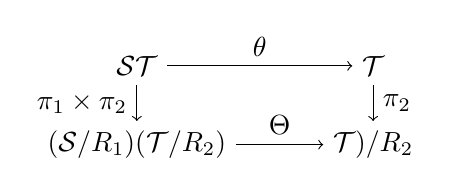
\begin{tikzpicture}
        \node (ST) at (0,0) {$\mathcal{S}\ltimes\mathcal{T}$};
        \node (T) at ([shift={+(3,0)}]ST) {$\mathcal{T}$};
        \node (SRTR) at ([shift={+(0,-1)}]ST) {$(\mathcal{S}/R_1)\ltimes(\mathcal{T}/R_2)$};
        \node (TR) at ([shift={+(0,-1)}]T) {$\mathcal{T})/R_2$};
        \draw[->] (ST)--(T) node[midway,above] {$\theta$};
        \draw[->] (ST)--(SRTR) node[midway,left] {$\pi_1\times\pi_2$};
        \draw[->] (T)--(TR) node[midway,right] {$\pi_2$};
        \draw[->] (SRTR)--(TR) node[midway,above] {$\Theta$};
    \end{tikzpicture}\]
    where the horizontal arrows are the action maps and the vertical ones are topological quotient maps. Since $\theta$ is continuous and open then $\Theta$ is continuous and open.\qedhere
    \end{enumerate}
\end{proof}

\begin{theorem}
Assuming hypotheses \ref{hyp:onrelationsforsemidirectproduct1} and \ref{hyp:onrelationsforsemidirectproduct2}, that $\mathcal{S}$ is étale, $\mathcal{T}$ is topological, $(\pi,\theta)$ is a continuous open $\land$-preaction, and that $R_1$ and $R_2$ are open, the map
\[\Phi\colon(\mathcal{S}\ltimes\mathcal{T})/(R_1\times R_2)\to(\mathcal{S}/R_1)\ltimes(\mathcal{T}/R_2),\qquad\Phi([a,x])=([a],[x])\]
is a topological semigroupoid isomorphism.
\end{theorem}
\begin{proof}
    The fact that $\Phi$ is a semigroupoid isomorphism is immediate. To check that it is also a homeomorphism, consider the commutative diagram
    \[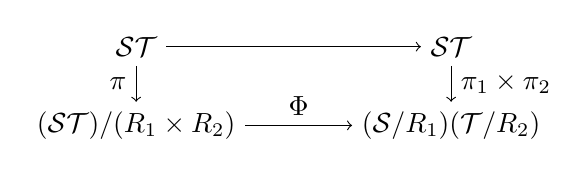
\begin{tikzpicture}
        \node (1ST) at (0,0) {$\mathcal{S}\ltimes\mathcal{T}$};
        \node (SRTR) at ([shift={+(0,-1)}]1ST) {$(\mathcal{S}/R_1)\ltimes(\mathcal{T}/R_2)$};
        \node (2ST) at ([shift={+(-4,0)}]1ST) {$\mathcal{S}\ltimes\mathcal{T}$};
        \node (STRR) at ([shift={+(0,-1)}]2ST) {$(\mathcal{S}\ltimes\mathcal{T})/(R_1\times R_2)$};
        \draw[->] (2ST)--(1ST) node[midway,above] {$\id$};
        \draw[->] (1ST)--(SRTR) node[midway,right] {$\pi_1\times\pi_2$};
        \draw[->] (2ST)--(STRR) node[midway,left] {$\pi$};
        \draw[->] (STRR)--(SRTR) node[midway,above] {$\Phi$};
    \end{tikzpicture}\]
    where $\pi_1$, $\pi_2$ and $\pi$ are canonical quotient maps. The vertical arrows are topological quotient maps, so and $\id$ is continuous and open, therefore $\Phi$ is continuous and open as well, hence a homeomorphism.\qedhere
\end{proof}

\subsection{Global actions}

In this subsection, let us consider global open actions of étale inverse semigroupoids on sets.

\begin{example}\label{ex:actiononvertexspace}
Every étale inverse semigroupoid $\mathcal{S}$ admits a canonical continuous, open action on its vertex space.

Let $\id_{\mathcal{S}^{(0)}}\colon\mathcal{S}^{(0)}\to\mathcal{S}^{(0)}$ be the trivial bundle. Define  $\tau\colon\mathcal{S}\to\mathcal{I}(\id_{\mathcal{S}^{(0)}})$ as $\tau_a(\so(a))=\ra(a)$ for all $a\in\mathcal{S}^{(0)}$ (that is, $\dom(\tau_a)=\left\{\so(a)\right\}$ and $\ran(\tau_a)=\left\{\ra(a)\right\})$.

As $\mathcal{S}$ is étale, it is easy to verify that $\mathbb{T}(\mathcal{S})\defeq(\id_{\mathcal{S}^{(0)}},\tau)$ is a continuous open action.
\end{example}

Denote by $\cat{Act}$ the category of continuous open actions of étale inverse semigroupoids on topological spaces. A morphism between actions $(\pi^i,\theta^i)\colon\mathcal{S}_i\curvearrowright X_i$ ($i=1,2$) is a pair $(f,\phi)$, where $f\colon X_1\to X_2$ is a continuous function and $\phi\colon\mathcal{S}_1\to\mathcal{S}_2$ is a continuous homomorphism, which are equivariant in the sense that for all $a\in\mathcal{S}$, $f\circ\theta^1_a\leq \theta^2_{\phi(a)}\circ f$ (i.e., $\theta^2_{\phi(a)}\circ f$ is an extension of $f\circ\theta_1^a$).

The composition of two morphisms is simply $(f_1,\phi_1)(f_2,\phi_2)=(f_1\circ f_2,\phi_1\circ\phi_2)$.

We will construct a pair of adjunct functors between $\cat{Act}$ and $\cat{EtIS}$. Let us denote by $\mathbb{T}(\mathcal{S})=(\id_{\mathcal{S}^{(0)}},\tau)$ the action constructed in Example \ref{ex:actiononvertexspace}, for an étale inverse semigroupoid $\mathcal{S}$. We already know that any continuous étale semigroupoid homomorphism $\phi\colon\mathcal{S}_1\to\mathcal{S}_2$ induces a continuous map on the vertex sets $\phi^{(0)}\colon\mathcal{S}_1^{(0)}\to\mathcal{S}_2^{(0)}$, by $\phi^{(0)}(\so(a))=\so(\phi(a))$. It is easy to see that $\mathbb{T}(\phi)\defeq(\phi^{(0)},\phi)$ is equivariant, and thus a morphism between the actions $\mathbb{T}(\mathcal{S}_1)$ and $\mathbb{T}(\mathcal{S}_2)$. We thus have a functor $\mathbb{T}\colon\cat{EtIS}\to\cat{Act}$.

In the other direction, given a morphism $(f,\phi)\colon(\pi_1,\theta_1)\to(\pi_2,\theta_2)$ of continuous open actions $(\pi_i,\theta_i)\colon\mathcal{S}_i\curvearrowright \mathcal{T}_i$, we define a continuous semigroupoid homomorphism $\ast(f,\phi)\colon\mathcal{S}_1\ltimes\mathcal{T}_1\to\mathcal{S}_2\ltimes \mathcal{T}_2$ by
\[\ast(f,\phi)(a,x)=(\phi(a),f(x)).\]
Therefore we have a functor $\ast\colon\cat{Act}\to\cat{EtIS}$, taking any action to the associated semidirect product.

\begin{proposition}
$(\mathbb{T},\ast)$ is a pair of adjoint functors. Moreover, $\ast\mathbb{T}$ is (naturally isomorphic to) the identity of $\cat{EtIS}$.
\end{proposition}
\begin{proof}
    We first define a natural transformation $\epsilon\colon\mathbb{T}\ast\to\id_{\cat{Act}}$. Given an action $(\pi,\theta)\colon\mathcal{S}\curvearrowright\mathcal{T}$, consider the homomorphism $\epsilon^{(1)}\colon\mathcal{S}\ast\mathcal{T}\to \mathcal{S}$, $\epsilon^{(1)}(a,x)=a$. Since the vertex set $(\mathcal{S}\ltimes X)^{(0)}$ is (a subset of) $X$, let $\epsilon^{(0)}\defeq\id_X$. Then $\epsilon_{(\pi,\theta)}=(\epsilon^{(0)},\epsilon^{(1)})$ is a morphism of actions, and this defines a natural transformation $\epsilon\colon \mathbb{T}\ast\to\id_{\cat{Act}}$.
    
    In the other direction, given an inverse semigroupoid $\mathcal{S}$, consider $\eta_{\mathcal{S}}\colon\mathcal{S}\to\mathcal{S}\ast\mathcal{S}^{(0)}$ as $\eta_{\mathcal{S}}(a)=(a,\so(a))$. Then $\eta_{\mathcal{S}}$ is actually an isomorphism, and this defines a natural isomorphism $\eta\colon\id_{\cat{EtIS}}\to\ast\mathbb{T}$.
    
    Elementary, although long, computations prove that $(\epsilon,\eta)$ is an adjunction between $\mathbb{T}$ and $\ast$.\qedhere
\end{proof}